\documentclass[12pt,english,pdf,xcolor=dvipsnames,aspectratio=169,handout]{beamer}\usepackage[]{graphicx}\usepackage[]{xcolor}
% maxwidth is the original width if it is less than linewidth
% otherwise use linewidth (to make sure the graphics do not exceed the margin)
\makeatletter
\def\maxwidth{ %
  \ifdim\Gin@nat@width>\linewidth
    \linewidth
  \else
    \Gin@nat@width
  \fi
}
\makeatother

\definecolor{fgcolor}{rgb}{0.345, 0.345, 0.345}
\newcommand{\hlnum}[1]{\textcolor[rgb]{0.686,0.059,0.569}{#1}}%
\newcommand{\hlstr}[1]{\textcolor[rgb]{0.192,0.494,0.8}{#1}}%
\newcommand{\hlcom}[1]{\textcolor[rgb]{0.678,0.584,0.686}{\textit{#1}}}%
\newcommand{\hlopt}[1]{\textcolor[rgb]{0,0,0}{#1}}%
\newcommand{\hlstd}[1]{\textcolor[rgb]{0.345,0.345,0.345}{#1}}%
\newcommand{\hlkwa}[1]{\textcolor[rgb]{0.161,0.373,0.58}{\textbf{#1}}}%
\newcommand{\hlkwb}[1]{\textcolor[rgb]{0.69,0.353,0.396}{#1}}%
\newcommand{\hlkwc}[1]{\textcolor[rgb]{0.333,0.667,0.333}{#1}}%
\newcommand{\hlkwd}[1]{\textcolor[rgb]{0.737,0.353,0.396}{\textbf{#1}}}%
\let\hlipl\hlkwb

\usepackage{framed}
\makeatletter
\newenvironment{kframe}{%
 \def\at@end@of@kframe{}%
 \ifinner\ifhmode%
  \def\at@end@of@kframe{\end{minipage}}%
  \begin{minipage}{\columnwidth}%
 \fi\fi%
 \def\FrameCommand##1{\hskip\@totalleftmargin \hskip-\fboxsep
 \colorbox{shadecolor}{##1}\hskip-\fboxsep
     % There is no \\@totalrightmargin, so:
     \hskip-\linewidth \hskip-\@totalleftmargin \hskip\columnwidth}%
 \MakeFramed {\advance\hsize-\width
   \@totalleftmargin\z@ \linewidth\hsize
   \@setminipage}}%
 {\par\unskip\endMakeFramed%
 \at@end@of@kframe}
\makeatother

\definecolor{shadecolor}{rgb}{.97, .97, .97}
\definecolor{messagecolor}{rgb}{0, 0, 0}
\definecolor{warningcolor}{rgb}{1, 0, 1}
\definecolor{errorcolor}{rgb}{1, 0, 0}
\newenvironment{knitrout}{}{} % an empty environment to be redefined in TeX

\usepackage{alltt}
\usepackage{etex}
\usetheme{default}
\beamertemplatenavigationsymbolsempty
\definecolor{fore}{RGB}{249,242,215}
\definecolor{back}{RGB}{51,51,51}
\definecolor{title}{RGB}{255,0,90}
\setbeamercolor{titlelike}{fg=title}
\setbeamercolor{normal text}{fg=fore,bg=back}
\setbeamertemplate{footline}[page number]
\usepackage{mathpazo}
\usepackage{amsmath}
\usepackage{multirow}
\renewcommand{\familydefault}{\rmdefault}
\usepackage[T1]{fontenc}
\usepackage{inputenc}
\usepackage{parskip}
\setcounter{secnumdepth}{3}
\setcounter{tocdepth}{3}
\usepackage{hyperref}
\hypersetup{pdfauthor={Constantin Manuel Bosancianu},
pdftitle={Event History Analysis in R},
pdfsubject={Introduction to event history analysis},
pdfkeywords={Heidelberg, survival analysis, day 2, slides}}
\usepackage{babel}
\usepackage{graphicx}
\usepackage[makeroom]{cancel}
\usepackage{pgfplots}
\pgfplotsset{compat=1.10}
\usepgfplotslibrary{fillbetween}
\usepackage{palatino}
% Defines a checkmark
\def\checkmark{\tikz\fill[scale=0.4,color=title](0,.35) -- (.25,0) -- (1,.7) -- (.25,.15) -- cycle;}
\setbeamertemplate{itemize items}{\checkmark}
% For table captions in Beamer
\usepackage{caption}
\captionsetup[figure]{labelfont={color=fore}}
\captionsetup[table]{labelfont={color=fore}}
\usepackage{tikz, tikz-cd, animate}
\usetikzlibrary{arrows,shapes,backgrounds,trees}
\usetikzlibrary{decorations.pathreplacing}
\usepackage{pgfplots}
\usepackage{pgfplotstable}
\usepackage{wrapfig}
\usepackage{booktabs}
\usepackage{dcolumn}
\usepackage[sectionbib]{apacite}
\renewcommand{\bibliographytypesize}{\footnotesize}
\title{Event History Analysis in R}
\subtitle{Day 2: Multivariate Analyses}
\author{Constantin Manuel Bosancianu}
\institute{Doctoral School of Political Science \\ Central European University, Budapest \\ \href{mailto:bosancianu@icloud.com}{bosancianu@icloud.com}}
\date{November 3, 2015}
\IfFileExists{upquote.sty}{\usepackage{upquote}}{}
\begin{document}
\maketitle




\section{Introduction}



\begin{frame}{Outline}
Yesterday was more theoretical - basic concepts in survival analysis, and a few descriptive summaries of the data.\bigskip

Today I'll try going for an ambitious target.\bigskip

\begin{itemize}
\item Cox Proportional Hazards (Cox PH) model
\item Investigating the PH assumption
\item Going past the PH assumption\footnote{Stratified Cox PH model and the extended Cox model.}
\end{itemize}

\end{frame}



\begin{frame}{Reason}
Why is Cox PH so important?\bigskip

Without giving away too much of the ending, it should be said that it's the ``OLS model'' of survival analysis:\bigskip

\begin{itemize}
\item Simple in its mechanics
\item Robust to slight violations in its assumptions (particularly the PH one)\footnote{There are a few other benefits, but it's best to leave them until we get to that section.}
\item Much better than a logistic regression model, because it uses information on survival time as well
\end{itemize}

\end{frame}




\section{Cox PH}

\begin{frame}

\begin{center}
\huge Cox Proportional Hazards model
\end{center}
\end{frame}



\begin{frame}{Cox PH model}
So far, we've been able to compare survivor probabilities and hazard rates between distinct groups in our sample (e.g. men vs. women, countries from South America vs. everywhere else).\bigskip

The Cox PH model is intended to provide additional controls when judging these relationships, since it can estimate hazard rates for groups in the sample, \textit{after adjusting for any number of categorical and continuous time-invariant predictors}.\bigskip

Roughly speaking, the Cox PH model is to the log-rank test what OLS regression is to the t-test.
\end{frame}



\begin{frame}{Cox PH model}
Let's use $X$ to denote a set (vector) of independent variables, $X_1$, $X_2$, \dots $X_k$.\bigskip

The formula for the Cox PH model is

\begin{equation}
  \centering
  h(t,X)=h_0(t) \times e^{\sum\limits_{i=1}^k\beta_i \times X_i}
\end{equation}
\bigskip

The model estimates the hazard rate for an individual at time t, based on a ``baseline hazard function'', $h_0(t)$, and the values on the vector of independent variables.
\end{frame}



\begin{frame}{Cox PH model}
Two interesting features of the model:

\begin{itemize}
\item $h_0(t)$ is a function that depends on time, but not on the $X$s
\item $e^{\sum\limits_{i=1}^k\beta_i \times X_i}$ depends on the $X$s, but not on time\footnote{The $X$s for now are time-invariant variables, e.g. the continent location for a country. If you want to use time-variant variables as well, the PH assumption no longer holds (``extended'' Cox model).}
\end{itemize}
\bigskip

If $X_1=X_2=\dots=X_k=0$, then $h(t,X)=h_0(t) \times e^0=h_0(t)$, which is why it's called the ``baseline function''.
\end{frame}



\begin{frame}{The baseline function}
$h_0(t)$ is interesting in itself--it can take any functional form.

\begin{figure}
\centering
\begin{tikzpicture}
 \begin{axis}[smooth,
    area style,
    width=6cm, height=4cm,xmin=0,xmax=4.5,ymin=0,ymax=1.2,
    no markers,
    samples=50,
    axis y line=left,
    axis x line=bottom,
    scale only axis,
    ytick={0,0.2,0.4,0.6,0.8,1},
    yticklabels={0,0.2,0.4,0.6,0.8,1},
    ylabel={$h(t)$},
    ylabel style={rotate=-90},
    xtick={0,2,4.5},
    xticklabels={0, t, $\infty$}
  ]
\addplot [const plot, no marks, thick, red] coordinates {(0,0.47) (4,0.47)};
  \end{axis}
\end{tikzpicture}
\caption*{Constant hazard function}
\end{figure}
  
\end{frame}




\begin{frame}{The baseline function}
  
\begin{figure}
\centering
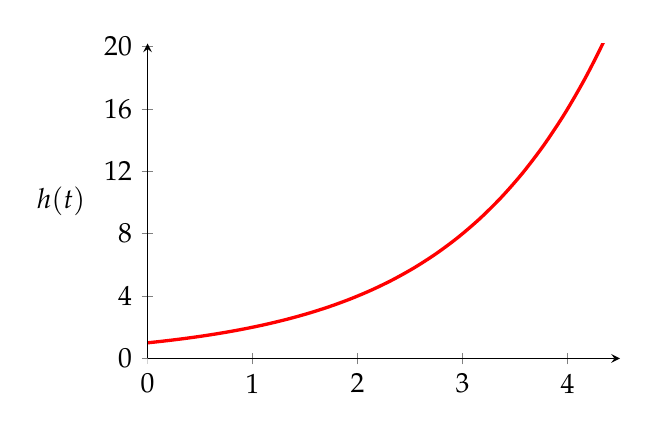
\begin{tikzpicture}
 \begin{axis}[smooth,
    area style,
    width=6cm, height=4cm,xmin=0,xmax=4.5,ymin=0,ymax=20.2,
    no markers,
    samples=50,
    axis y line=left,
    axis x line=bottom,
    scale only axis,
    ytick={0,4,8,12,16,20},
    yticklabels={0,4,8,12,16,20},
    ylabel={$h(t)$},
    ylabel style={rotate=-90},
    xtick={0,1,2,3,4},
    xticklabels={0,1,2,3,4}
  ]
\addplot[red, very thick]  {pow(2,x)} node[above, midway, xshift=-1cm] {};
  \end{axis}
\end{tikzpicture}
\caption*{Weibull hazard function}
\end{figure}

Other functions are also possible, such as the decreasing Weibull, or the lognormal.
\end{frame}



\begin{frame}{The baseline function}
Because of its ability to handle multiple forms for the baseline hazard function, the Cox PH model is a ``semiparametric'' model.\bigskip

Other benefits (apart from those mentioned already):

\begin{itemize}
\item Due to its robustness, it's a ``safe'' choice \cite[p.~111]{Kleinbaum2012}
\item The exponential part guarantees we never get negative predicted hazard rates, which are mathematically impossible
\end{itemize}

\end{frame}



\subsection{Estimates}
\begin{frame}{Estimates}
No point in going into the estimation procedure which is a flavour of Maximum Likelihood (partial ML).\bigskip

The estimates that you get from the model, though, are (indirectly) hazard ratios.\bigskip

\begin{equation}
\centering
\widehat{HR}=\frac{\widehat{h}(t,X^{*})}{\widehat{h}(t,X^{\dagger})}
\end{equation}

Here, $X^{*}$ and $X^{\dagger}$ denote two sets of values on the explanatory variables for two observations.
\end{frame}



\begin{frame}{Estimates}
Let's say that $X^{*}=1$ denotes a country from Latin America from my data set, while $X^{\dagger}=0$ refers to all other countries.\bigskip

\begin{equation}
  \centering
  \widehat{HR}=\frac{\widehat{h}(t,X^{*})}{\widehat{h}(t,X^{\dagger})}=\frac{\cancel{\widehat{h}_0^{*}(t)} \times e^{\sum\limits_{i=1}^k\hat{\beta}_i \times X_i^{*}}}{\cancel{\widehat{h}_0^{\dagger}(t)} \times e^{\sum\limits_{i=1}^k\hat{\beta}_i \times X_i^{\dagger}}}
\end{equation}

Essentially, the Cox PH model needs the PH assumption for those hazard functions to cancel each other out. The baseline hazard is not even estimated.\footnote{Because of the PH assumption, $h_0^{*}=h_0^{\dagger} \times \theta$, where $\theta$ is a constant. The $\theta$ disappears as well when we take the logarithm of the quantity.}
\end{frame}



\begin{frame}{Estimates}

\begin{equation}
  \centering
  \widehat{HR}=\frac{e^{\sum\limits_{i=1}^k\hat{\beta}_i \times X_i^{*}}}{e^{\sum\limits_{i=1}^k\hat{\beta}_i \times X_i^{\dagger}}}=e^{\sum\limits_{i=1}^{k}\hat{\beta}_i(X_i^{*} - X_i^{\dagger})}
\end{equation}

In my case, $X^{*}=1$ and  $X^{\dagger}=0$, which means the equation reduces to $\widehat{HR}=e^{\beta}$.\bigskip

The coefficients we get from the model are the $\beta$s, but we can get to hazard ratios by computing $e^{\beta}$ and thus getting the hazard ratio.
\end{frame}



\begin{frame}{Hazard ratios}
They are like ``odds ratios'' in logistic regression. A HR larger than one denotes a higher hazard rate for the first group than the second.\bigskip

Suppose the coefficient in my model would have been 2. $\widehat{HR}$=7.3890561, which means drug users would be at a much higher risk of dying compared to non-users.\bigskip

If $\beta>0$, the $HR>1$. If $\beta<0$, then $HR<1$.

\end{frame}


\subsection{Practical Cox PH}

\begin{frame}[fragile]{Practical Cox PH}
I won't use the same data as yesterday; it's a sexy topic, but I couldn't get any model to show something interesting \textit{and} statistically significant.\bigskip

Today we'll rely on a data set \cite<from>{HosmerJr1999} comprised of 100 HIV infected persons, tracking their survival time.\bigskip

\begin{knitrout}\scriptsize
\definecolor{shadecolor}{rgb}{0.969, 0.969, 0.969}\color{fgcolor}\begin{kframe}
\begin{alltt}
\hlstd{path} \hlkwb{<-} \hlstr{"https://stats.idre.ucla.edu/stat/r/examples/asa/hmohiv.csv"}
\hlstd{hmohiv} \hlkwb{<-} \hlkwd{read.table}\hlstd{(path,} \hlkwc{sep} \hlstd{=} \hlstr{","}\hlstd{,} \hlkwc{header} \hlstd{=} \hlnum{TRUE}\hlstd{)}
\end{alltt}
\end{kframe}
\end{knitrout}

\end{frame}



\begin{frame}[fragile]{Practical Cox PH}
\begin{knitrout}\scriptsize
\definecolor{shadecolor}{rgb}{0.969, 0.969, 0.969}\color{fgcolor}\begin{kframe}
\begin{alltt}
\hlstd{hmohiv |>}
  \hlkwd{glimpse}\hlstd{()}
\end{alltt}
\begin{verbatim}
Rows: 100
Columns: 7
$ ID      <int> 1, 2, 3, 4, 5, 6, 7, 8, 9, 10, 11, 12, 13, 14, 15, 16, 17, 18,~
$ time    <int> 5, 6, 8, 3, 22, 1, 7, 9, 3, 12, 2, 12, 1, 15, 34, 1, 4, 19, 3,~
$ age     <int> 46, 35, 30, 30, 36, 32, 36, 31, 48, 47, 28, 34, 44, 32, 36, 36~
$ drug    <int> 0, 1, 1, 1, 0, 1, 1, 1, 0, 0, 1, 0, 1, 1, 0, 0, 0, 0, 1, 0, 0,~
$ censor  <int> 1, 0, 1, 1, 1, 0, 1, 1, 1, 1, 0, 1, 1, 1, 1, 1, 1, 0, 0, 1, 0,~
$ entdate <chr> "5/15/1990 ", "9/19/1989 ", "4/21/1991 ", "1/3/1991 ", "9/18/1~
$ enddate <chr> "10/14/1990 ", "3/20/1990 ", "12/20/1991 ", "4/4/1991 ", "7/19~
\end{verbatim}
\end{kframe}
\end{knitrout}

\end{frame}



\begin{frame}[fragile]{Practical Cox PH}

\begin{knitrout}\scriptsize
\definecolor{shadecolor}{rgb}{0.969, 0.969, 0.969}\color{fgcolor}\begin{kframe}
\begin{alltt}
\hlkwd{library}\hlstd{(Zelig)}
\hlstd{z.out} \hlkwb{<-} \hlkwd{zelig}\hlstd{(}\hlkwd{Surv}\hlstd{(time, censor)} \hlopt{~} \hlstd{drug} \hlopt{+} \hlstd{age,}
               \hlkwc{model} \hlstd{=} \hlstr{"coxph"}\hlstd{,} \hlkwc{data} \hlstd{= hmohiv)}
\end{alltt}
\end{kframe}
\end{knitrout}
\bigskip

Unfortunately, the model does not work in \texttt{Zelig}, although it was available in previous versions (e.g. 3.5.x).\bigskip

Keep following it, though, it's bound to appear again soon.
\end{frame}



\begin{frame}[fragile]{Practical Cox PH: \texttt{survival}}
\begin{knitrout}\tiny
\definecolor{shadecolor}{rgb}{0.969, 0.969, 0.969}\color{fgcolor}\begin{kframe}
\begin{alltt}
\hlkwd{colnames}\hlstd{(hmohiv)[}\hlnum{5}\hlstd{]} \hlkwb{<-} \hlstr{"death"} \hlcom{# the variable name was odd}
\hlstd{model.1} \hlkwb{<-} \hlkwd{coxph}\hlstd{(}\hlkwd{Surv}\hlstd{(time, death)} \hlopt{~} \hlstd{drug} \hlopt{+} \hlstd{age,} \hlkwc{data} \hlstd{= hmohiv)}
\hlkwd{summary}\hlstd{(model.1)}
\end{alltt}
\begin{verbatim}
Call:
coxph(formula = Surv(time, death) ~ drug + age, data = hmohiv)

  n= 100, number of events= 80 

        coef exp(coef) se(coef)     z Pr(>|z|)    
drug 1.01670   2.76405  0.25622 3.968 7.24e-05 ***
age  0.09714   1.10202  0.01864 5.211 1.87e-07 ***
---
Signif. codes:  0 '***' 0.001 '**' 0.01 '*' 0.05 '.' 0.1 ' ' 1

     exp(coef) exp(-coef) lower .95 upper .95
drug     2.764     0.3618     1.673     4.567
age      1.102     0.9074     1.062     1.143

Concordance= 0.711  (se = 0.033 )
Likelihood ratio test= 39.13  on 2 df,   p=3e-09
Wald test            = 36.13  on 2 df,   p=1e-08
Score (logrank) test = 38.39  on 2 df,   p=5e-09
\end{verbatim}
\end{kframe}
\end{knitrout}

\texttt{Surv()} creates the \texttt{survival} object which is used as a response variable in the analysis.
\end{frame}



\begin{frame}[fragile]{Practical Cox PH: \texttt{survival}}
Breaking down the results for the drug use dummy indicator.\bigskip

\begin{itemize}
\item \texttt{coef}=1.0166984 is the estimated coefficient (a logged hazard ratio) for the dummy indicator;
\item \texttt{exp(coef)}=2.7640538 is the hazard ratio for the variable;
\item \texttt{se(coef)}=0.256217 is the standard error for the \underline{coefficient};
\item \texttt{z}=3.9681137 is the z value ($\frac{\beta}{SE}$);
\item \texttt{Pr(>|z|)}=\ensuremath{7.2443761\times 10^{-5}} is the p value associated with the coefficient.
\end{itemize}

\end{frame}



\begin{frame}{Practical Cox PH: \texttt{survival}}
The output presents a range of other pieces of information.\bigskip

\begin{itemize}
\item Lower and upper CIs for the hazard ratio;
\item LR test: compare the model with a null model (the baseline hazard rate) in terms of fit;
\item $R^2$ value for the model fit (a Nagelkerke type of $R^2$).
\end{itemize}
\bigskip
Wald test is generally considered less reliable than the LR one.
\end{frame}



\begin{frame}{Model fit: \texttt{concordance}}
\texttt{Concordance} is a specific measure for the Cox PH model.\bigskip

It denotes the percentage of pairs (A,B) of observations where the hazard of A is greater than that of B, and A gets the event before B.\bigskip

It isn't very accurate through: it doesn't indicate \textit{by how much sooner} A gets the event faster than B.
\end{frame}



\begin{frame}[fragile]{Cox PH: predictions}
We could also obtain expected hazard ratios, with the \texttt{predict()} function.\bigskip

\begin{knitrout}\scriptsize
\definecolor{shadecolor}{rgb}{0.969, 0.969, 0.969}\color{fgcolor}\begin{kframe}
\begin{alltt}
\hlkwd{predict}\hlstd{(model.1,} \hlkwc{type} \hlstd{=} \hlstr{"risk"}\hlstd{,} \hlkwc{se.fit} \hlstd{=} \hlnum{TRUE}\hlstd{)} \hlcom{# hazard ratio}
\hlkwd{predict}\hlstd{(model.1,} \hlkwc{type} \hlstd{=} \hlstr{"lp"}\hlstd{,} \hlkwc{se.fit} \hlstd{=} \hlnum{TRUE}\hlstd{)} \hlcom{# linear predictor}
\hlkwd{predict}\hlstd{(model.1,} \hlkwc{type} \hlstd{=} \hlstr{"expected"}\hlstd{,} \hlkwc{se.fit} \hlstd{=} \hlnum{TRUE}\hlstd{)}
\hlcom{# expected number of events}
\end{alltt}
\end{kframe}
\end{knitrout}

The linear predictor is the $\sum\limits_{i=1}^{i}\beta_{i}X_{i}$ quantity. Predictions of the ``expected'' type incorporate the baseline hazard rate as well.
\end{frame}



\begin{frame}[fragile]{Cox PH: predictions}
We can also plot expected survival rates for particular ``types'' of individual in the data.\bigskip





\begin{knitrout}\scriptsize
\definecolor{shadecolor}{rgb}{0.969, 0.969, 0.969}\color{fgcolor}\begin{kframe}
\begin{alltt}
\hlkwd{plot}\hlstd{(}\hlkwd{survfit}\hlstd{(model.1,} \hlkwc{newdata} \hlstd{=} \hlkwd{data.frame}\hlstd{(}\hlkwc{drug} \hlstd{=} \hlnum{1}\hlstd{,} \hlkwc{age} \hlstd{=} \hlnum{50}\hlstd{)),}
     \hlkwc{xlab} \hlstd{=} \hlstr{"Time"}\hlstd{,} \hlkwc{ylab} \hlstd{=} \hlstr{"Survival"}\hlstd{)}
\end{alltt}
\end{kframe}
\end{knitrout}

\begin{figure}
\centering
\includegraphics[width=0.45\textwidth]{../03-graphs/02-01}
\includegraphics[width=0.45\textwidth]{../03-graphs/02-02}
\caption*{Left: \texttt{age}=20. Right: \texttt{age}=40. Comparison for drug users.}
\end{figure}
\end{frame}



\begin{frame}[fragile]{Cox PH: predictions}
An alternative is the \texttt{simPH} package, which essentially fills the gap which \texttt{Zelig} left.\bigskip

\begin{knitrout}\scriptsize
\definecolor{shadecolor}{rgb}{0.969, 0.969, 0.969}\color{fgcolor}\begin{kframe}
\begin{alltt}
\hlkwd{library}\hlstd{(simPH)}
\hlstd{hmohiv} \hlkwb{<-} \hlstd{hmohiv |>} \hlkwd{mutate}\hlstd{(}\hlkwc{cent_age} \hlstd{= age} \hlopt{-} \hlkwd{mean}\hlstd{(age,} \hlkwc{na.rm} \hlstd{=} \hlnum{TRUE}\hlstd{))}
\hlstd{model.2} \hlkwb{<-} \hlkwd{coxph}\hlstd{(}\hlkwd{Surv}\hlstd{(time, death)} \hlopt{~} \hlstd{drug} \hlopt{+} \hlstd{cent_age,} \hlkwc{data} \hlstd{= hmohiv)}
\hlstd{sim.2} \hlkwb{<-} \hlkwd{coxsimLinear}\hlstd{(model.2,} \hlkwc{b} \hlstd{=} \hlstr{"cent_age"}\hlstd{,} \hlkwc{Xj} \hlstd{=} \hlkwd{seq}\hlstd{(}\hlopt{-}\hlnum{10}\hlstd{,} \hlnum{8}\hlstd{,} \hlkwc{by} \hlstd{=} \hlnum{0.25}\hlstd{),}
                      \hlkwc{nsim} \hlstd{=} \hlnum{250}\hlstd{)}
\hlcom{# The smaller the "by=" interval, the smoother the graph}
\hlkwd{simGG}\hlstd{(sim.2,} \hlkwc{xlab} \hlstd{=} \hlstr{"Centered age"}\hlstd{,} \hlkwc{type} \hlstd{=} \hlstr{"lines"}\hlstd{)}
\end{alltt}
\end{kframe}
\end{knitrout}



\end{frame}



\begin{frame}[fragile]{Cox PH: predictions}

\begin{figure}
\centering
\includegraphics[width=0.75\textwidth]{../03-graphs/02-03}
\end{figure}
\end{frame}



\begin{frame}[fragile]{Cox PH: predictions}

\begin{knitrout}\scriptsize
\definecolor{shadecolor}{rgb}{0.969, 0.969, 0.969}\color{fgcolor}\begin{kframe}
\begin{alltt}
\hlstd{sim.3} \hlkwb{<-} \hlkwd{coxsimLinear}\hlstd{(model.2,} \hlkwc{b} \hlstd{=} \hlstr{"drug"}\hlstd{,} \hlkwc{Xj} \hlstd{=} \hlnum{0}\hlopt{:}\hlnum{1}\hlstd{,}
                      \hlkwc{nsim} \hlstd{=} \hlnum{250}\hlstd{)}
\hlstd{graph2} \hlkwb{<-} \hlkwd{simGG}\hlstd{(sim.3,} \hlkwc{xlab} \hlstd{=} \hlstr{"Drug use"}\hlstd{,} \hlkwc{type} \hlstd{=} \hlstr{"lines"}\hlstd{,} \hlkwc{method} \hlstd{=} \hlstr{"lm"}\hlstd{)}
\hlstd{graph2} \hlopt{+} \hlkwd{scale_x_continuous}\hlstd{(}\hlkwc{limits} \hlstd{=} \hlkwd{c}\hlstd{(}\hlnum{0}\hlstd{,} \hlnum{1}\hlstd{),}
    \hlkwc{breaks} \hlstd{=} \hlkwd{c}\hlstd{(}\hlnum{0}\hlstd{,} \hlnum{1}\hlstd{),} \hlkwc{labels} \hlstd{=} \hlkwd{c}\hlstd{(}\hlstr{"No drug use"}\hlstd{,} \hlstr{"Drug use"}\hlstd{))}
\end{alltt}
\end{kframe}
\end{knitrout}



The option \texttt{method=``lm''} is needed to make sure that the lines are straight, and don't get smoothed.\bigskip

The \texttt{simGG()} function produces a \texttt{ggplot2} object, so we can modify a lot of things about it.\footnote{Remember the cool graph themes available in the \texttt{ggthemes} package.}

\end{frame}



\begin{frame}[fragile]{Cox PH: predictions}
We can obtain similar predictions for dichotomous variables.\bigskip

\begin{figure}
\centering
\includegraphics[width=0.65\textwidth]{../03-graphs/02-04}
\end{figure}
\end{frame}



\section{The PH assumption}

\begin{frame}

\begin{center}
\huge Assessing the PH assumption
\end{center}
\end{frame}



\begin{frame}{PH assumption}
The assumption can be checked, to see if the Cox PH model is appropriate under the circumstances.\bigskip

Three ways of checking:
\begin{itemize}
\item Graphically (through log--log curves)
\item Through a goodness-of-fit (GOF) test
\item Relying on time-dependent variables
\end{itemize}
\end{frame}



\subsection{Graphical checks}
\begin{frame}{PH check: graphical}
What we want to see is parallel log--log curves: $ln(-ln(\widehat{S}))$.\bigskip

$\widehat{S} \in (0;1)$, which means $-ln(\widehat{S}) \in (0;\infty)$, which means $ln(-ln(\widehat{S})) \in (-\infty; \infty)$.\bigskip

We have a hazard function from the Cox model, which we can convert to a survival function through some mathematical trasformations.
\end{frame}


\begin{frame}{PH check: graphical}

\begin{figure}
\centering
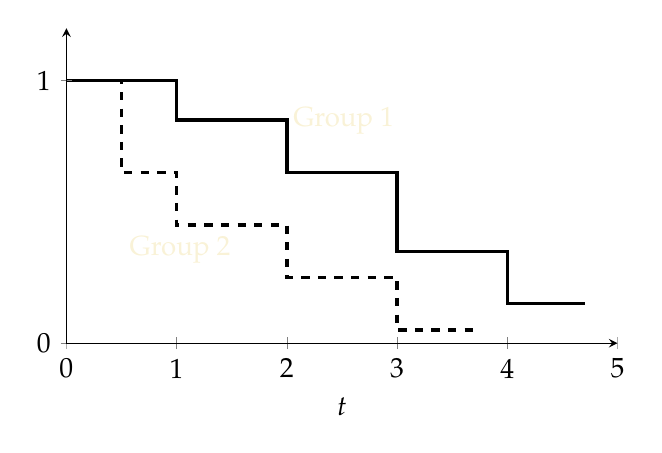
\begin{tikzpicture}
 \begin{axis}[smooth,
    area style,
    width=7cm, height=4cm,xmin=0,xmax=5,ymin=0,ymax=1.2,
    no markers,
    samples=50,
    axis y line=left,
    axis x line=bottom,
    scale only axis,
    ytick={0,1},
%    ylabel={$S(t)$},
%    ylabel style={rotate=-90},
    xlabel={$t$}
  ]
\addplot [const plot, no marks, very thick] coordinates {(0,1) (1,1) (1,0.85) (2,0.85) (2,0.65) (3,0.65) (3,0.35) (4,0.35) (4, 0.15) (4.7,0.15)} node[right,pos=0.38,fore] {Group 1};
\addplot [const plot, no marks, very thick, dashed] coordinates {(0,1) (0.5,1) (0.5,0.65) (1,0.65) (1,0.45) (2,0.45) (2,0.25) (3,0.25) (3, 0.05) (3.7,0.05)} node[below,pos=0.34,fore] {Group 2};
  \end{axis}
\end{tikzpicture}
\caption*{Roughly parallel lines mean the PH assumption is met}
\end{figure}
\end{frame}



\begin{frame}{PH check: graphical}

\begin{figure}
\centering
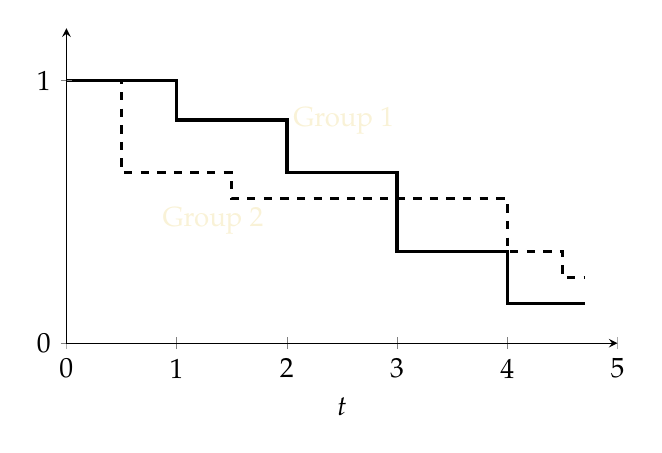
\begin{tikzpicture}
 \begin{axis}[smooth,
    area style,
    width=7cm, height=4cm,xmin=0,xmax=5,ymin=0,ymax=1.2,
    no markers,
    samples=50,
    axis y line=left,
    axis x line=bottom,
    scale only axis,
    ytick={0,1},
%    ylabel={$S(t)$},
%    ylabel style={rotate=-90}.
    xlabel={$t$}
  ]
\addplot [const plot, no marks, very thick] coordinates {(0,1) (1,1) (1,0.85) (2,0.85) (2,0.65) (3,0.65) (3,0.35) (4,0.35) (4, 0.15) (4.7,0.15)} node[right,pos=0.38,fore] {Group 1};
\addplot [const plot, no marks, very thick, dashed] coordinates {(0,1) (0.5,1) (0.5,0.65) (1.5,0.65) (1.5,0.55) (2.5,0.55) (3.5,0.55) (4,0.45) (4, 0.35) (4.5,0.35) (4.5, 0.25) (4.7,0.25)} node[below,pos=0.34, xshift=-0.2cm, yshift=-0.3cm, fore] {Group 2};
  \end{axis}
\end{tikzpicture}
\caption*{Crossing, converging or diverging lines mean the PH assumption is not met}
\end{figure}
\end{frame}



\begin{frame}[fragile]{PH check: graphical}
Done for Kaplan-Meier survival estimates, one variable at a time.\bigskip

\begin{knitrout}\scriptsize
\definecolor{shadecolor}{rgb}{0.969, 0.969, 0.969}\color{fgcolor}\begin{kframe}
\begin{alltt}
\hlcom{# This is not a Cox PH model}
\hlstd{model.1} \hlkwb{<-} \hlkwd{survfit}\hlstd{(}\hlkwd{Surv}\hlstd{(time, death)} \hlopt{~} \hlstd{drug,} \hlkwc{data} \hlstd{= hmohiv)}
\hlkwd{plot}\hlstd{(model.1,} \hlkwc{fun} \hlstd{=} \hlstr{"cloglog"}\hlstd{,} \hlkwc{lty} \hlstd{=} \hlkwd{c}\hlstd{(}\hlstr{"solid"}\hlstd{,} \hlstr{"dashed"}\hlstd{),}
     \hlkwc{col} \hlstd{=} \hlkwd{c}\hlstd{(}\hlstr{"red"}\hlstd{,} \hlstr{"blue"}\hlstd{),} \hlkwc{xlab} \hlstd{=} \hlstr{"Time in log scale"}\hlstd{,}
     \hlkwc{ylab} \hlstd{=} \hlstr{"log-log survival"}\hlstd{)}
\end{alltt}
\end{kframe}
\end{knitrout}



\end{frame}



\begin{frame}[fragile]{PH check: graphical}

\begin{figure}
\centering
\includegraphics[width=0.7\textwidth]{../03-graphs/02-05.pdf}
\caption*{The PH assumption appears to be satisfied with respect to drug use}
\end{figure}
\end{frame}



\begin{frame}[fragile]{PH check: graphical}
We can follow the same strategy with respect to continuous variables, but we have to split them into $k$ categories.\bigskip

\begin{knitrout}\scriptsize
\definecolor{shadecolor}{rgb}{0.969, 0.969, 0.969}\color{fgcolor}\begin{kframe}
\begin{alltt}
\hlkwd{quantile}\hlstd{(hmohiv}\hlopt{$}\hlstd{age,} \hlkwd{c}\hlstd{(}\hlnum{0.33}\hlstd{,} \hlnum{0.66}\hlstd{))} \hlcom{# find ages at those precise}
\hlcom{# locations in the age distribution}
\hlstd{hmohiv}\hlopt{$}\hlstd{agecat[hmohiv}\hlopt{$}\hlstd{age} \hlopt{<=} \hlnum{32}\hlstd{]} \hlkwb{<-} \hlnum{0}
\hlstd{hmohiv}\hlopt{$}\hlstd{agecat[hmohiv}\hlopt{$}\hlstd{age} \hlopt{>=} \hlnum{33} \hlopt{&} \hlstd{hmohiv}\hlopt{$}\hlstd{age} \hlopt{<=} \hlnum{38}\hlstd{]} \hlkwb{<-} \hlnum{1}
\hlstd{hmohiv}\hlopt{$}\hlstd{agecat[hmohiv}\hlopt{$}\hlstd{age} \hlopt{>=} \hlnum{39}\hlstd{]} \hlkwb{<-} \hlnum{2}
\hlstd{model.1} \hlkwb{<-} \hlkwd{survfit}\hlstd{(}\hlkwd{Surv}\hlstd{(time, death)} \hlopt{~} \hlstd{agecat,} \hlkwc{data} \hlstd{= hmohiv)}
\hlkwd{plot}\hlstd{(model.1,} \hlkwc{fun} \hlstd{=} \hlstr{"cloglog"}\hlstd{,} \hlkwc{lty} \hlstd{=} \hlkwd{c}\hlstd{(}\hlstr{"solid"}\hlstd{,} \hlstr{"dashed"}\hlstd{,} \hlstr{"dotted"}\hlstd{),}
     \hlkwc{col} \hlstd{=} \hlkwd{c}\hlstd{(}\hlstr{"red"}\hlstd{,} \hlstr{"blue"}\hlstd{,} \hlstr{"green"}\hlstd{),} \hlkwc{xlab} \hlstd{=} \hlstr{"Time in log scale"}\hlstd{,}
     \hlkwc{ylab} \hlstd{=} \hlstr{"log-log survival"}\hlstd{)}
\end{alltt}
\end{kframe}
\end{knitrout}



It's good to choose a manageable number of categories, e.g. 2 or 3.
\end{frame}



\begin{frame}[fragile]{PH check: graphical}

\begin{figure}
\centering
\includegraphics[width=0.7\textwidth]{../03-graphs/02-06.pdf}
\caption*{The PH assumption appears to be satisfied with respect to age too}
\end{figure}
\end{frame}



\begin{frame}[fragile]{Graphical checks: problems}
The graphical check approach has a few inherent problems \cite[pp.~172--174]{Kleinbaum2012}:\bigskip

\begin{itemize}
\item Deciding whether lines are parallel is a subjective decision
\item Deciding how to split variables into groups is also subjective
\item Difficult strategy with reduced samples (some groups could be very small)
\end{itemize}
\end{frame}



\begin{frame}[fragile]{PH check: graphical}
A second graphical approach is to plot expected vs. observed survival curves.\bigskip

First stage involves running a Cox PH model and obtaining expected curves based on the values of the predictor.\bigskip

The second stage is to obtain Kaplan--Meier curves as we did above.\bigskip

We then plot the two sets of curves and inspect how closely they overlap.
\end{frame}



\subsection{GOF approach}
\begin{frame}{GOF checks}
They are appealing, because they provide a single digit, with an associated \textit{p} value, on the basis of which to make a decision.\bigskip

Based on Schoenfeld residuals, which is computed for each observation which experiences an event, for each of the DVs in the model.\bigskip

Residuals are computed as $X_i - weighted(X_{\sim i})$, where $X_i$ is observation's $i$ value on the $X$ variable, $X_{\sim i}$ are the values for all other observations, and the weights are those observations' hazard rates.
\end{frame}



\begin{frame}{GOF checks: procedure}
Three-stage procedure:\bigskip

\begin{itemize}
\item Compute Schoenfeld residuals for each observation
\item Construct a variable that orders survival times, from lowest to highest
\item Correlate this variable with the residuals
\end{itemize}
\bigskip

If PH assumption is valid, there should be no correlation observed.
\end{frame}



\begin{frame}[fragile]{GOF checks: procedure}
R does all of this for you automatically, with a slight twist: it uses scaled Schoenfeld residuals.\footnote{In the vast majority of cases, the results should be the same. The scaling procedure involves adjusting the residuals by the covariance matrix of the residuals.} \bigskip

\begin{knitrout}\scriptsize
\definecolor{shadecolor}{rgb}{0.969, 0.969, 0.969}\color{fgcolor}\begin{kframe}
\begin{alltt}
\hlstd{model.1} \hlkwb{<-} \hlkwd{coxph}\hlstd{(}\hlkwd{Surv}\hlstd{(time, death)} \hlopt{~} \hlstd{drug} \hlopt{+} \hlstd{age,} \hlkwc{data} \hlstd{= hmohiv)}
\hlkwd{cox.zph}\hlstd{(model.1,} \hlkwc{transform} \hlstd{=} \hlstr{"km"}\hlstd{,} \hlkwc{global} \hlstd{=} \hlnum{FALSE}\hlstd{)}
\end{alltt}
\begin{verbatim}
        chisq df    p
drug 0.000158  1 0.99
age  0.017640  1 0.89
\end{verbatim}
\begin{alltt}
\hlcom{# The "global" option does a global chi-square test}
\hlcom{# in addition to one for each variable.}
\end{alltt}
\end{kframe}
\end{knitrout}

We want to see low correlations ($\rho$), and $p$ values above 0.05.
\end{frame}


\subsection{Time-dependent}
\begin{frame}{Time-dependent checks}
The procedure involves using a function of time, and interacting this with the predictors.\bigskip

If the PH assumption is valid, the coefficient on the interaction should not be statistically significant.\bigskip

\begin{equation}
  \centering
  h(t,X)=h_0(t) \times e^{\beta X + \delta (X \times g(t))}
\end{equation}

$g(t)=t$, or $g(t)=log(t)$, or many others.
\end{frame}



\begin{frame}[fragile]{Time-dependent checks: \texttt{R}}
\begin{knitrout}\scriptsize
\definecolor{shadecolor}{rgb}{0.969, 0.969, 0.969}\color{fgcolor}\begin{kframe}
\begin{alltt}
\hlstd{model.2} \hlkwb{<-} \hlkwd{coxph}\hlstd{(}\hlkwd{Surv}\hlstd{(time, death)} \hlopt{~} \hlstd{drug} \hlopt{+} \hlstd{age} \hlopt{+} \hlkwd{tt}\hlstd{(drug),} \hlkwc{data} \hlstd{= hmohiv,}
                 \hlkwc{tt}\hlstd{=}\hlkwa{function}\hlstd{(}\hlkwc{x}\hlstd{,} \hlkwc{t}\hlstd{,} \hlkwc{...}\hlstd{) x} \hlopt{*} \hlstd{t)}
\end{alltt}
\end{kframe}
\end{knitrout}

The function I chose here is simply $g(t)=t$.\bigskip

The model has to be run with the \texttt{tt} argument. If you try computing by hand a $drug \times time$ interaction, the model will have convergence errors due to multicollinearity.

\end{frame}



\begin{frame}[fragile]{Time-dependent checks: \texttt{R}}
\begin{knitrout}\tiny
\definecolor{shadecolor}{rgb}{0.969, 0.969, 0.969}\color{fgcolor}\begin{kframe}
\begin{alltt}
\hlkwd{summary}\hlstd{(model.2);} \hlkwd{rm}\hlstd{(model.2)}
\end{alltt}
\begin{verbatim}
Call:
coxph(formula = Surv(time, death) ~ drug + age + tt(drug), data = hmohiv, 
    tt = function(x, t, ...) x * t)

  n= 100, number of events= 80 

             coef exp(coef) se(coef)      z Pr(>|z|)    
drug      1.19633   3.30796  0.34992  3.419 0.000629 ***
age       0.09487   1.09951  0.01892  5.013 5.35e-07 ***
tt(drug) -0.02828   0.97212  0.03878 -0.729 0.465940    
---
Signif. codes:  0 '***' 0.001 '**' 0.01 '*' 0.05 '.' 0.1 ' ' 1

         exp(coef) exp(-coef) lower .95 upper .95
drug        3.3080     0.3023     1.666     6.568
age         1.0995     0.9095     1.059     1.141
tt(drug)    0.9721     1.0287     0.901     1.049

Concordance= 0.708  (se = 0.034 )
Likelihood ratio test= 39.81  on 3 df,   p=1e-08
Wald test            = 36.35  on 3 df,   p=6e-08
Score (logrank) test = 38.95  on 3 df,   p=2e-08
\end{verbatim}
\end{kframe}
\end{knitrout}

\end{frame}



\section{Stratified Cox model}

\begin{frame}

\begin{center}
\huge Stratified Cox model
\end{center}
\end{frame}



\begin{frame}{Stratification}
An extension to the case when one of the variables is clearly shown not to abide by the PH assumption.\bigskip

The solution essentially involves running models separately for each category of the variable--stratifying based on the variable.\bigskip

Unfortunately, everything was pretty good with the previous model, so there's not much we can do there.
\end{frame}



\begin{frame}{Alternative data}
\begin{table}
\centering
\scriptsize
\begin{tabular}{l l l}
\toprule
Variable & Description & Values \\
\midrule
ID & Identification code & 1-628\\
AGE & Age at enrollment & Years \\
BECKTOTA & Beck depression score at admission & 0-54 \\
HERCOC & Heroin/cocaine use during 3 & 1=both; 2=only heroin; \\
       & months prior to admission   & 3=only cocaine; 4=neither \\
IVHX & Drug use history at admission & 1=never; 2=previous; 3=recent \\
NDRUGTX & No. of prior drug treatments & 0-40 \\
RACE & Subject's race & 0=White; 1=other \\
TREAT & Treatment randomization & 0=short; 1=long \\
SITE & Treatment site & 0=A; 1=B \\
LOT & Length of treatment & No. of days \\
TIME & Time to return to drug use & No. of days\footnote{Measured starting from admission time.} \\
CENSOR & Returned to drug use & 1=yes; 0=otherwise \\
\bottomrule
\end{tabular}
\end{table}
\end{frame}



\begin{frame}[fragile]{Stratification}
\begin{knitrout}\scriptsize
\definecolor{shadecolor}{rgb}{0.969, 0.969, 0.969}\color{fgcolor}\begin{kframe}
\begin{alltt}
\hlstd{df_uis} \hlkwb{<-} \hlkwd{read.table}\hlstd{(}\hlstr{"../02-data/03-uissurv.dat"}\hlstd{,} \hlkwc{quote} \hlstd{=} \hlstr{"\textbackslash{}""}\hlstd{,}
                     \hlkwc{comment.char} \hlstd{=} \hlstr{""}\hlstd{)}
\hlstd{df_uis} \hlkwb{<-} \hlstd{df_uis |>}
  \hlkwd{rename}\hlstd{(}\hlkwc{id} \hlstd{=} \hlnum{1}\hlstd{,} \hlkwc{age} \hlstd{=} \hlnum{2}\hlstd{,} \hlkwc{becktota} \hlstd{=} \hlnum{3}\hlstd{,} \hlkwc{hercoc} \hlstd{=} \hlnum{4}\hlstd{,} \hlkwc{ivhx} \hlstd{=} \hlnum{5}\hlstd{,}
         \hlkwc{ndrugtx} \hlstd{=} \hlnum{6}\hlstd{,} \hlkwc{race} \hlstd{=} \hlnum{7}\hlstd{,} \hlkwc{treat} \hlstd{=} \hlnum{8}\hlstd{,} \hlkwc{site} \hlstd{=} \hlnum{9}\hlstd{,} \hlkwc{lot} \hlstd{=} \hlnum{10}\hlstd{,}
         \hlkwc{time} \hlstd{=} \hlnum{11}\hlstd{,} \hlkwc{censor} \hlstd{=} \hlnum{12}\hlstd{) |>}
  \hlkwd{mutate}\hlstd{(}\hlkwc{becktota} \hlstd{=} \hlkwd{if_else}\hlstd{(becktota} \hlopt{==} \hlstr{"."}\hlstd{,} \hlnum{NA_character_}\hlstd{, becktota),}
         \hlkwc{hercoc} \hlstd{=} \hlkwd{if_else}\hlstd{(hercoc} \hlopt{==} \hlstr{"."}\hlstd{,} \hlnum{NA_character_}\hlstd{, hercoc),}
         \hlkwc{ivhx} \hlstd{=} \hlkwd{if_else}\hlstd{(ivhx} \hlopt{==} \hlstr{"."}\hlstd{,} \hlnum{NA_character_}\hlstd{, ivhx),}
         \hlkwc{race} \hlstd{=} \hlkwd{if_else}\hlstd{(race} \hlopt{==} \hlstr{"."}\hlstd{,} \hlnum{NA_character_}\hlstd{, race),}
         \hlkwc{age} \hlstd{=} \hlkwd{if_else}\hlstd{(age} \hlopt{==} \hlstr{"."}\hlstd{,} \hlnum{NA_character_}\hlstd{, age)) |>}
  \hlkwd{mutate_at}\hlstd{(}\hlkwc{.vars} \hlstd{=} \hlkwd{vars}\hlstd{(becktota, hercoc, ivhx, race, age),}
            \hlkwc{.funs} \hlstd{= as.numeric)}
\hlstd{model.3} \hlkwb{<-} \hlkwd{coxph}\hlstd{(}\hlkwd{Surv}\hlstd{(time, censor)} \hlopt{~} \hlstd{age} \hlopt{+} \hlstd{becktota} \hlopt{+} \hlstd{ivhx} \hlopt{+} \hlstd{treat} \hlopt{+}
                   \hlstd{site} \hlopt{+} \hlstd{lot,} \hlkwc{data} \hlstd{= df_uis,} \hlkwc{na.action} \hlstd{= na.omit)}
\end{alltt}
\end{kframe}
\end{knitrout}

\end{frame}



\begin{frame}[fragile]{Stratification}
\begin{knitrout}\tiny
\definecolor{shadecolor}{rgb}{0.969, 0.969, 0.969}\color{fgcolor}\begin{kframe}
\begin{verbatim}
Call:
coxph(formula = Surv(time, censor) ~ age + becktota + ivhx + 
    treat + site + lot, data = df_uis, na.action = na.omit)

  n= 591, number of events= 475 
   (37 observations deleted due to missingness)

               coef  exp(coef)   se(coef)       z Pr(>|z|)    
age      -0.0196807  0.9805117  0.0079033  -2.490   0.0128 *  
becktota  0.0040371  1.0040453  0.0047896   0.843   0.3993    
ivhx      0.3014561  1.3518257  0.0570247   5.286 1.25e-07 ***
treat     0.1520115  1.1641736  0.0942117   1.614   0.1066    
site      0.4972081  1.6441247  0.1071282   4.641 3.46e-06 ***
lot      -0.0092848  0.9907582  0.0008012 -11.588  < 2e-16 ***
---
Signif. codes:  0 '***' 0.001 '**' 0.01 '*' 0.05 '.' 0.1 ' ' 1

         exp(coef) exp(-coef) lower .95 upper .95
age         0.9805     1.0199    0.9654    0.9958
becktota    1.0040     0.9960    0.9947    1.0135
ivhx        1.3518     0.7397    1.2089    1.5117
treat       1.1642     0.8590    0.9679    1.4003
site        1.6441     0.6082    1.3327    2.0283
lot         0.9908     1.0093    0.9892    0.9923

Concordance= 0.735  (se = 0.011 )
Likelihood ratio test= 180.9  on 6 df,   p=<2e-16
Wald test            = 159.6  on 6 df,   p=<2e-16
Score (logrank) test = 162.4  on 6 df,   p=<2e-16
\end{verbatim}
\end{kframe}
\end{knitrout}

\end{frame}



\begin{frame}[fragile]{Stratification}
\begin{knitrout}\scriptsize
\definecolor{shadecolor}{rgb}{0.969, 0.969, 0.969}\color{fgcolor}\begin{kframe}
\begin{alltt}
\hlkwd{cox.zph}\hlstd{(model.3,} \hlkwc{transform} \hlstd{=} \hlstr{"km"}\hlstd{,} \hlkwc{global} \hlstd{=} \hlnum{FALSE}\hlstd{)}
\end{alltt}
\begin{verbatim}
           chisq df      p
age        0.299  1 0.5847
becktota   2.575  1 0.1085
ivhx       0.038  1 0.8455
treat      9.882  1 0.0017
site       3.046  1 0.0809
lot      207.034  1 <2e-16
\end{verbatim}
\end{kframe}
\end{knitrout}

We clearly have a problem here with the \texttt{length of treatment} variable.
\end{frame}



\begin{frame}[fragile]{Stratified Cox}
The model is a simple variation on the standard Cox model.\bigskip

\begin{equation}
\centering
h_g(t,X) = {h_0}_g(t) \times e^{\sum\limits_{i=1}^{k}\beta_iX_i}
\end{equation}

Here \texttt{g} designates the strata. We have separate baseline hazards for the different categories (strata).
\end{frame}



\begin{frame}[fragile]{Stratified Cox: practical}
A simple extension of the \texttt{R} code as well.\bigskip

\begin{knitrout}\scriptsize
\definecolor{shadecolor}{rgb}{0.969, 0.969, 0.969}\color{fgcolor}\begin{kframe}
\begin{alltt}
\hlkwd{quantile}\hlstd{(df_uis}\hlopt{$}\hlstd{lot,} \hlkwd{c}\hlstd{(}\hlnum{0.33}\hlstd{,} \hlnum{0.66}\hlstd{))} \hlcom{# examine cutoff points}
\end{alltt}
\begin{verbatim}
  33%   66% 
55.00 94.82 
\end{verbatim}
\begin{alltt}
\hlstd{df_uis}\hlopt{$}\hlstd{lotcat[df_uis}\hlopt{$}\hlstd{lot} \hlopt{<} \hlnum{55}\hlstd{]} \hlkwb{<-} \hlnum{0}
\hlstd{df_uis}\hlopt{$}\hlstd{lotcat[df_uis}\hlopt{$}\hlstd{lot} \hlopt{>=} \hlnum{55} \hlopt{&} \hlstd{df_uis}\hlopt{$}\hlstd{lot} \hlopt{<=} \hlnum{94}\hlstd{]} \hlkwb{<-} \hlnum{1}
\hlstd{df_uis}\hlopt{$}\hlstd{lotcat[df_uis}\hlopt{$}\hlstd{lot} \hlopt{>} \hlnum{94}\hlstd{]} \hlkwb{<-} \hlnum{2}
\hlstd{model.4} \hlkwb{<-} \hlkwd{coxph}\hlstd{(}\hlkwd{Surv}\hlstd{(time, censor)} \hlopt{~} \hlstd{age} \hlopt{+} \hlstd{becktota} \hlopt{+} \hlstd{ivhx} \hlopt{+} \hlstd{treat} \hlopt{+}
                   \hlstd{site} \hlopt{+} \hlkwd{strata}\hlstd{(lotcat),} \hlkwc{data} \hlstd{= df_uis,} \hlkwc{na.action} \hlstd{= na.omit)}
\end{alltt}
\end{kframe}
\end{knitrout}
\end{frame}



\begin{frame}[fragile]{Stratified Cox: practical}
\begin{knitrout}\tiny
\definecolor{shadecolor}{rgb}{0.969, 0.969, 0.969}\color{fgcolor}\begin{kframe}
\begin{verbatim}
Call:
coxph(formula = Surv(time, censor) ~ age + becktota + ivhx + 
    treat + site + strata(lotcat), data = df_uis, na.action = na.omit)

  n= 591, number of events= 475 
   (37 observations deleted due to missingness)

              coef exp(coef)  se(coef)      z Pr(>|z|)    
age      -0.021194  0.979029  0.008056 -2.631  0.00852 ** 
becktota  0.005115  1.005128  0.004791  1.068  0.28563    
ivhx      0.242769  1.274774  0.056782  4.275 1.91e-05 ***
treat     0.020763  1.020980  0.100144  0.207  0.83575    
site      0.210432  1.234211  0.112827  1.865  0.06217 .  
---
Signif. codes:  0 '***' 0.001 '**' 0.01 '*' 0.05 '.' 0.1 ' ' 1

         exp(coef) exp(-coef) lower .95 upper .95
age          0.979     1.0214    0.9637    0.9946
becktota     1.005     0.9949    0.9957    1.0146
ivhx         1.275     0.7845    1.1405    1.4248
treat        1.021     0.9795    0.8390    1.2424
site         1.234     0.8102    0.9894    1.5397

Concordance= 0.559  (se = 0.014 )
Likelihood ratio test= 24.2  on 5 df,   p=2e-04
Wald test            = 24.01  on 5 df,   p=2e-04
Score (logrank) test = 24.13  on 5 df,   p=2e-04
\end{verbatim}
\end{kframe}
\end{knitrout}

\end{frame}


\begin{frame}[fragile]{Stratified Cox: practical}
Each stratum will have the same coefficients on the $\beta$s, but their baseline hazard rates are probably different. \bigskip

\begin{knitrout}\tiny
\definecolor{shadecolor}{rgb}{0.969, 0.969, 0.969}\color{fgcolor}\begin{kframe}
\begin{alltt}
\hlkwd{plot}\hlstd{(}\hlkwd{survfit}\hlstd{(model.4))}
\end{alltt}
\end{kframe}
\end{knitrout}



\begin{figure}
\centering
\includegraphics[width=0.6\textwidth]{../03-graphs/02-07.pdf}
\end{figure}
\end{frame}



\begin{frame}[fragile]{Stratified Cox: practical}
The ``un-stratified'' model will make no such distinction between basic hazard rates.\bigskip

\begin{knitrout}\tiny
\definecolor{shadecolor}{rgb}{0.969, 0.969, 0.969}\color{fgcolor}\begin{kframe}
\begin{alltt}
\hlkwd{plot}\hlstd{(}\hlkwd{survfit}\hlstd{(model.3))}
\end{alltt}
\end{kframe}
\end{knitrout}



\begin{figure}
\centering
\includegraphics[width=0.6\textwidth]{../03-graphs/02-08.pdf}
\end{figure}
\end{frame}



\begin{frame}[fragile]{Stratified Cox}
With multiple variables, they are added in the same \texttt{strata} field, e.g. \texttt{strata(IV1+IV2+...)}.\bigskip

R will create categories based on them, e.g. 2 categories for \texttt{IV1} and 3 for \texttt{IV2} $\Rightarrow$ 6 categories.\bigskip

\underline{Assumption}: there is no interaction between strata and the estimated parameters: ${\beta_1}_{(1)}={\beta_1}_{(2)}={\beta_1}_{(3)}={\beta_1}_{(4)}=\dots$
\end{frame}



\begin{frame}[fragile]{Stratified Cox}
It's safe to test the assumption, with a series of interactions.\bigskip

\begin{knitrout}\scriptsize
\definecolor{shadecolor}{rgb}{0.969, 0.969, 0.969}\color{fgcolor}\begin{kframe}
\begin{alltt}
\hlkwd{rm}\hlstd{(model.3, model.4)}
\hlcom{# Recode the LoT variable into only two categories, for convenience}
\hlkwd{quantile}\hlstd{(df_uis}\hlopt{$}\hlstd{lot,} \hlnum{0.5}\hlstd{)} \hlcom{# median is 84}
\end{alltt}
\begin{verbatim}
50% 
 84 
\end{verbatim}
\begin{alltt}
\hlstd{df_uis} \hlkwb{<-} \hlstd{df_uis |>} \hlkwd{mutate}\hlstd{(}\hlkwc{lotcat} \hlstd{=} \hlkwd{if_else}\hlstd{(lot} \hlopt{<} \hlnum{84}\hlstd{,} \hlnum{0}\hlstd{,} \hlnum{1}\hlstd{))}
\hlcom{# Model with stratification}
\hlstd{model.4.1} \hlkwb{<-} \hlkwd{coxph}\hlstd{(}\hlkwd{Surv}\hlstd{(time, censor)} \hlopt{~} \hlstd{age} \hlopt{+} \hlstd{becktota} \hlopt{+} \hlstd{ivhx} \hlopt{+} \hlstd{treat} \hlopt{+}
                     \hlstd{site} \hlopt{+} \hlkwd{strata}\hlstd{(lotcat),} \hlkwc{data} \hlstd{= df_uis,} \hlkwc{na.action} \hlstd{= na.omit)}
\hlcom{# Model with interactions}
\hlstd{model.4.2} \hlkwb{<-} \hlkwd{coxph}\hlstd{(}\hlkwd{Surv}\hlstd{(time, censor)} \hlopt{~} \hlstd{age} \hlopt{+} \hlstd{becktota} \hlopt{+} \hlstd{ivhx} \hlopt{+} \hlstd{treat} \hlopt{+}
                     \hlstd{site} \hlopt{+} \hlstd{age} \hlopt{*} \hlstd{lotcat} \hlopt{+} \hlstd{becktota} \hlopt{*} \hlstd{lotcat} \hlopt{+} \hlstd{ivhx} \hlopt{*} \hlstd{lotcat} \hlopt{+}
                     \hlstd{treat} \hlopt{*} \hlstd{lotcat} \hlopt{+} \hlstd{site} \hlopt{*} \hlstd{lotcat,} \hlkwc{data} \hlstd{= df_uis,}
                   \hlkwc{na.action} \hlstd{= na.omit)}
\end{alltt}
\end{kframe}
\end{knitrout}
\end{frame}


\begin{frame}[fragile]{Stratified Cox}
\begin{knitrout}\scriptsize
\definecolor{shadecolor}{rgb}{0.969, 0.969, 0.969}\color{fgcolor}\begin{kframe}
\begin{alltt}
\hlkwd{round}\hlstd{(}\hlkwd{summary}\hlstd{(model.4.1)}\hlopt{$}\hlstd{coefficients,}
      \hlkwc{digits} \hlstd{=} \hlnum{3}\hlstd{)}
\end{alltt}
\begin{verbatim}
           coef exp(coef) se(coef)      z Pr(>|z|)
age      -0.019     0.981    0.008 -2.394    0.017
becktota  0.007     1.007    0.005  1.437    0.151
ivhx      0.261     1.298    0.057  4.595    0.000
treat    -0.144     0.866    0.093 -1.543    0.123
site      0.079     1.082    0.106  0.741    0.459
\end{verbatim}
\end{kframe}
\end{knitrout}
\end{frame}


\begin{frame}[fragile]{Stratified Cox}
\begin{knitrout}\scriptsize
\definecolor{shadecolor}{rgb}{0.969, 0.969, 0.969}\color{fgcolor}\begin{kframe}
\begin{alltt}
\hlkwd{round}\hlstd{(}\hlkwd{summary}\hlstd{(model.4.2)}\hlopt{$}\hlstd{coefficients,}
      \hlkwc{digits} \hlstd{=} \hlnum{3}\hlstd{)}
\end{alltt}
\begin{verbatim}
                  coef exp(coef) se(coef)      z Pr(>|z|)
age             -0.042     0.959    0.012 -3.584    0.000
becktota         0.004     1.004    0.007  0.594    0.552
ivhx             0.433     1.543    0.084  5.154    0.000
treat            0.088     1.092    0.133  0.661    0.509
site             0.608     1.837    0.152  3.992    0.000
lotcat          -1.299     0.273    0.548 -2.371    0.018
age:lotcat       0.035     1.036    0.016  2.214    0.027
becktota:lotcat  0.005     1.005    0.010  0.506    0.613
ivhx:lotcat     -0.242     0.785    0.115 -2.105    0.035
treat:lotcat    -0.359     0.698    0.187 -1.921    0.055
site:lotcat     -0.788     0.455    0.210 -3.750    0.000
\end{verbatim}
\end{kframe}
\end{knitrout}
\end{frame}



\begin{frame}[fragile]{Stratified Cox}
Likelihood ratio (LR) test: $-2*LL_{M2} - (-2*LL_{M1})$ is distributed $\chi^2$, with $k_{M2} - k_{M1}$ degrees of freedom, where $k$ is the number of predictors of the models.\bigskip

\begin{knitrout}\scriptsize
\definecolor{shadecolor}{rgb}{0.969, 0.969, 0.969}\color{fgcolor}\begin{kframe}
\begin{alltt}
\hlkwd{lrtest}\hlstd{(model.4.1, model.4.2)}
\end{alltt}
\begin{verbatim}
Likelihood ratio test

Model 1: Surv(time, censor) ~ age + becktota + ivhx + treat + site + strata(lotcat)
Model 2: Surv(time, censor) ~ age + becktota + ivhx + treat + site + age * 
    lotcat + becktota * lotcat + ivhx * lotcat + treat * lotcat + 
    site * lotcat
  #Df  LogLik Df  Chisq Pr(>Chisq)    
1   5 -2387.5                         
2  11 -2664.1  6 553.18  < 2.2e-16 ***
---
Signif. codes:  0 '***' 0.001 '**' 0.01 '*' 0.05 '.' 0.1 ' ' 1
\end{verbatim}
\end{kframe}
\end{knitrout}

The coefficients do vary between strata.
\end{frame}



\section{Extended Cox model}


\begin{frame}

\begin{center}
\huge Extended Cox model
\end{center}
\end{frame}


\begin{frame}{Extended Cox}
We can partition the vector of coefficients into two:

\begin{itemize}
\item $X^{*}$ which only contains time-invariant variables: $X_1$, $X_2$, \dots $X_k$
\item $X^{\dagger}$ which only contains time-variant variables: $X_1(t)$, $X_2(t)$, \dots $X_j(t)$
\end{itemize}

\begin{equation}
\centering
h(t, X(t)) = h_0(t) \times e^{\sum\limits_{i=1}^{k} \beta X_i^{*} + \sum\limits_{i=1}^{j} \delta X_i^{\dagger}(t)}
\end{equation}

Even though $X_i^{\dagger}$ is time-variant, the estimated $\delta$ is the same for all time periods.
\end{frame}



\begin{frame}{\texttt{heart} data}

\begin{table}
\centering
\scriptsize
\begin{tabular}{l l l}
\toprule
Variable & Description & Values \\
\midrule
START & Time at which program was entered & - \\
STOP & Time when program was exited & - \\
EVENT & Death status & 1=dead; 0=censored; \\
AGE & Age at acceptance into program & Years - 48 \\
YEAR & Year of acceptance & Year - Nov 1, 1967 \\
SURGERY & Previous surgery & 1=yes; 0=no \\
TRANSPLANT & If ind. had transplant & 1=yes; 2=no \\
\bottomrule
\end{tabular}
\caption*{Stanford Heart Transplant Study (1967-1974, N=103)}
\end{table}
\end{frame}



\begin{frame}[fragile]{Extended Cox: practical}
69 (67\%) patients received a transplant and 75 (73\%) patients died (45 recipients of new hearts and 30 non-recipients).\bigskip

There is a problem, though: people who died sooner never got the chance to get a transplant, since it takes time to find a donor.\bigskip

This might make transplants appear overly effective.
\end{frame}



\begin{frame}[fragile]{Extended Cox: practical}
The \texttt{heart} data is available in the \texttt{survival} package.\bigskip

\begin{knitrout}\scriptsize
\definecolor{shadecolor}{rgb}{0.969, 0.969, 0.969}\color{fgcolor}\begin{kframe}
\begin{alltt}
\hlkwd{data}\hlstd{(heart)}
\hlstd{heart |>} \hlkwd{glimpse}\hlstd{()}
\end{alltt}
\begin{verbatim}
Rows: 172
Columns: 8
$ start      <dbl> 0, 0, 0, 1, 0, 36, 0, 0, 0, 51, 0, 0, 0, 12, 0, 26, 0, 0, 1~
$ stop       <dbl> 50, 6, 1, 16, 36, 39, 18, 3, 51, 675, 40, 85, 12, 58, 26, 1~
$ event      <dbl> 1, 1, 0, 1, 0, 1, 1, 1, 0, 1, 1, 1, 0, 1, 0, 1, 1, 0, 1, 0,~
$ age        <dbl> -17.15537303, 3.83572895, 6.29705681, 6.29705681, -7.737166~
$ year       <dbl> 0.1232033, 0.2546201, 0.2655715, 0.2655715, 0.4900753, 0.49~
$ surgery    <dbl> 0, 0, 0, 0, 0, 0, 0, 0, 0, 0, 0, 0, 0, 0, 0, 0, 0, 0, 0, 0,~
$ transplant <fct> 0, 0, 0, 1, 0, 1, 0, 0, 0, 1, 0, 0, 0, 1, 0, 1, 0, 0, 1, 0,~
$ id         <dbl> 1, 2, 3, 3, 4, 4, 5, 6, 7, 7, 8, 9, 10, 10, 11, 11, 12, 13,~
\end{verbatim}
\end{kframe}
\end{knitrout}

We don't have a time variable, but \texttt{Surv()} can handle a beginning and end indicator, which we have in the data.
\end{frame}




\begin{frame}[fragile]{Extended Cox: practical}
We don't have to worry about clustering at the level of individual; the software knows what observation to pick for inclusion in the likelihood function.\bigskip

This is a new way of arranging the data, but it's the only way \texttt{survival} knows how to handle time-varying predictors.\bigskip

\begin{knitrout}\scriptsize
\definecolor{shadecolor}{rgb}{0.969, 0.969, 0.969}\color{fgcolor}\begin{kframe}
\begin{alltt}
\hlstd{model.5} \hlkwb{<-} \hlkwd{coxph}\hlstd{(}\hlkwd{Surv}\hlstd{(start, stop, event)} \hlopt{~} \hlstd{transplant} \hlopt{+} \hlstd{surgery} \hlopt{+} \hlstd{age} \hlopt{+} \hlstd{year,}
                 \hlkwc{data} \hlstd{= heart)}
\end{alltt}
\end{kframe}
\end{knitrout}
\end{frame}


\begin{frame}[fragile]{Extended Cox: practical}
\begin{knitrout}\tiny
\definecolor{shadecolor}{rgb}{0.969, 0.969, 0.969}\color{fgcolor}\begin{kframe}
\begin{verbatim}
Call:
coxph(formula = Surv(start, stop, event) ~ transplant + surgery + 
    age + year, data = heart)

  n= 172, number of events= 75 

                coef exp(coef) se(coef)      z Pr(>|z|)  
transplant1 -0.01025   0.98980  0.31375 -0.033   0.9739  
surgery     -0.63721   0.52877  0.36723 -1.735   0.0827 .
age          0.02717   1.02754  0.01371  1.981   0.0476 *
year        -0.14635   0.86386  0.07047 -2.077   0.0378 *
---
Signif. codes:  0 '***' 0.001 '**' 0.01 '*' 0.05 '.' 0.1 ' ' 1

            exp(coef) exp(-coef) lower .95 upper .95
transplant1    0.9898     1.0103    0.5352    1.8307
surgery        0.5288     1.8912    0.2574    1.0860
age            1.0275     0.9732    1.0003    1.0555
year           0.8639     1.1576    0.7524    0.9918

Concordance= 0.636  (se = 0.033 )
Likelihood ratio test= 15.11  on 4 df,   p=0.004
Wald test            = 14.49  on 4 df,   p=0.006
Score (logrank) test = 15.03  on 4 df,   p=0.005
\end{verbatim}
\end{kframe}
\end{knitrout}

\end{frame}


\begin{frame}[fragile]{Extended Cox: practical}
\begin{knitrout}\scriptsize
\definecolor{shadecolor}{rgb}{0.969, 0.969, 0.969}\color{fgcolor}\begin{kframe}
\begin{alltt}
\hlcom{# Respondents of 38 years old, with no transplant}
\hlkwd{plot}\hlstd{(}\hlkwd{survfit}\hlstd{(model.5,} \hlkwc{newdata} \hlstd{=} \hlkwd{data.frame}\hlstd{(}\hlkwc{transplant} \hlstd{=} \hlnum{0}\hlstd{,} \hlkwc{age} \hlstd{=} \hlopt{-}\hlnum{10}\hlstd{,}
                                           \hlkwc{surgery} \hlstd{=} \hlnum{0}\hlstd{,} \hlkwc{year} \hlstd{=} \hlnum{0}\hlstd{)),}
     \hlkwc{xlab} \hlstd{=} \hlstr{"Time"}\hlstd{,} \hlkwc{ylab} \hlstd{=} \hlstr{"Survival"}\hlstd{)}
\hlcom{# Respondents of 68 years old, with no transplant}
\hlkwd{plot}\hlstd{(}\hlkwd{survfit}\hlstd{(model.5,} \hlkwc{newdata} \hlstd{=} \hlkwd{data.frame}\hlstd{(}\hlkwc{transplant} \hlstd{=} \hlnum{0}\hlstd{,} \hlkwc{age} \hlstd{=} \hlnum{20}\hlstd{,}
                                           \hlkwc{surgery} \hlstd{=} \hlnum{0}\hlstd{,} \hlkwc{year} \hlstd{=} \hlnum{0}\hlstd{)),}
     \hlkwc{xlab} \hlstd{=} \hlstr{"Time"}\hlstd{,} \hlkwc{ylab} \hlstd{=} \hlstr{"Survival"}\hlstd{)}
\end{alltt}
\end{kframe}
\end{knitrout}

Respondents are similar in other respects: no past experience of surgery, and admitted to the program in November 1967.



\end{frame}



\begin{frame}[fragile]{Extended Cox: practical}

\begin{figure}
\centering
\includegraphics[width=0.4\textwidth]{../03-graphs/02-09.pdf}
\includegraphics[width=0.4\textwidth]{../03-graphs/02-10.pdf}
\caption*{Left: \texttt{age}=38. Right: \texttt{age}=68.}
\end{figure}

Clearly, older individuals have lower survival rates.
\end{frame}



\section{Conclusion}

\begin{frame}{Concluding remarks}
The Cox PH model is quite a good choice for the initial steps in the analysis.\bigskip

It's robust, can accomodate a range of situations (some not covered here), and is relatively simple to run.\bigskip

Other more complex models await: accelerated failure time models (AFT), frailty models etc.
\end{frame}


\begin{frame}
\begin{center}
    \Huge Thank \textcolor{title}{you} for the kind attention!
\end{center}
\end{frame}

\begin{frame}{References}
\bibliographystyle{apacite}
\bibliography{../Bibliography}
\end{frame}

\end{document}
